% !TEX encoding = UTF-8 Unicode
%!TEX root = ../Main/thesis.tex
% !TEX spellcheck = en-US
%%=========================================
\documentclass[../Main/thesis.tex]{subfiles}
\begin{document}
\chapter{Technologies}
\label{ch:technologies}

Several technologies have been used for this project, and they can be divided into three categories, depending on the part of the system to witch they belongs: app, back end, and front end.
This chapter provides an overview of the technologies used in the research, and provides an explanation of how and why they where chosen and used.
It will also describe some alternative technologies that could have been used.
The intention is not to give a comprehensive presentation of the technologies, but instead give a brief introduction to support and explain the choices made.

\section{Bluetooth Low Energy Beacons}

\subsection{Bluetooth}
Bluetooth is a low-power, short-range wireless technology used to connect two or more devices together so they can share data such as images, audio and information between them \citep{bluetooth-how}.
Today Bluetooth-antennas are included in a wide range of electronic devices such as laptops, mobile phones and tablets.
There are two different radio version within the Bluetooth standard: Bluetooth Basic Rate/Enhanced Data Rate (BR/EDR), and Bluetooth Low Energy (LE) \citep{BluetoothSpecialInterestGroup2018}.
This project is utilizing the features of the Bluetooth Low Energy radio in small and easily movable beacons, or transmitters.

\subsection{Bluetooth Low Energy}
The Bluetooth Low Energy (BLE) standard is a subset of the Bluetooth standard.
It is designed for low power operation transmitting data in short bursts instead of continuous data streaming \citep{BluetoothSpecialInterestGroup2018}.
As \citet[p. 2]{Mackensen2012} explain ``BLE is a connection oriented wireless technology, i.e. two devices  which  want  to  exchange  data  must  enter  a  fixed connection before a data transmission is possible''.
%TODO write about states

\subsection{iBeacon protocol}
In 2013 Apple released the iBeacon protocol which is a wireless BLE protocol.
It is native to iOS, but it is also compatible with other devices such as Android.
A beacon using the iBeacon protocol will periodically broadcast a data packet consisting of three data points: Universally Unique Identifier (UUID), Major, and Minor \citep{Apple2014}.
Those data points are described in Table~\ref{tab:iBeacon-protocol}.

This data packet is received by other devices within its range. 
Those devices are then able to read the data and use it.

\begin{table}[h]
\centering
\caption[Description of iBeacon data packets]{Description of iBeacon data packets\citep[p. 3]{Apple2014}}
\begin{tabular}{|p{0.1\linewidth}|p{0.1\linewidth}|p{0.7\linewidth}|}
\hline
\textbf{Field} & \textbf{Size} & \textbf{Description}                                                                                                                       \\ \hline
\textbf{UUID}  & 16 bytes      & Application developers should define a UUID specific to their app and deployment use case.                                                 \\ \hline
\textbf{Major} & 2 bytes       & Further specifies a specific iBeacon and use case. For example, this could define a sub-region within a larger region defined by the UUID. \\ \hline
\textbf{Minor} & 2 bytes       & Allows further subdivision of region or use case, specified by the application developer.                                                  \\ \hline
\end{tabular}
\label{tab:iBeacon-protocol}
\end{table}

\section{Android application}
Android is the most used operating system for smartphones \citep{osmarketshare}. 
It is developed by Google and is based on the Linux kernel.
Android was initially released in 2005 \citep{Morrill2008a} and the most current version is Android 9 ``Pie'' \citep{Samat2018}.

The main alternative to using Android would be to use Apples iOS.
Since both had experience developing for Android and neither have developed for iOS earlier, Android was chosen to save time due to my familiarity with programming for Android.
Another reason for choosing Android is access to devices for testing (both have an Android)
A recommendation is that if you are developing for iOS you should use a Mac, to which we did not have access.

If the system was to be developed for commercial use the best choice would be to develop for both Android and iOS, but due to time limitations only the Android version will be developed. 
It is also outside the scope of our project.

There are a great variety of libraries available when developing applications for Android.
Some of these add new functionality and some simplify an existing task.
A few libraries used in FireTracker are described below. 

\subsection{Java}
Java is a programming language developed by Sun Microsystems in 1995 \citep{SunMicrosystems1996}. 
It is a general-purpose, concurrent, class-based and object-oriented language \citep[p. 1]{Gosling2018}.
Java code is compiled to bytecode which can run on a Java Virtual Machine (JVM) independent of computer architecture \citep{Venners2000}. 
Java is the most common language to use when developing applications for Android, which is the main reason for choosing it..
The other reason is that out of the three languages Java, Kotlin and C++ \citep{Google2018b} available for developing Android apps, Java is the only one we have prior experience with.


\subsection{Android Beacon Library}
Android Beacon Library (ABL) is an Android library that enables Android devices to interact with BLE beacons. 
It simplifies the process of searching for beacons and retrieve information, such as id, name and RSSI from them.
The library can also be used to listen for beacons in the background \citep{RadiusNetwork2015}.
This library was chosen because it is one of few libraries that is actively maintained.
It is also compatible with several different beacon-standards, and does not require proprietary beacons such as the Estimote SDK \citep{Estimote2017}.
This is an advantage because we are not limited to using only one beacon manufacturer or beacon type.

\subsection{Retrofit}
Retrofit is a type-safe HTTP client for Android and Java \citep{SquareInc.2017}.
This library was used to handle all HTTP requests from the app to the back end. 
It makes it easy to define your API endpoints as an interface in the app and send requests to the endpoint.
This results in consistency because the endpoints are used in the same way each time you use them, you cannot suddenly forget to add a required parameter one place in the code and remember it somewhere else.
Another benefit is that the code is more reusable, so the same code lines so not need to be written over and over again.
Retrofit also handles the response from the server and takes care of failures as well.

\subsection{Eventbus}
Eventbus is a library that makes it easier to send data between activities and threads in Android. 
It is simple to use.
Wherever you want to send data you post an ``event'' containing the data, and then you listen for the events where you want to use the data \citep{Greenrobot2016}.
This simplifies the common task of updating GUI-elements with data fetched from a server.
One of the alternatives to using Eventbus is storing all download data locally on the device and then reading the data from storage again when it is needed, this is both slower and more unstable as one cannot always be sure that the data is stored before you try to load it. 

\subsection{Butter Knife}
Butter Knife is a library for binding the user interface objects in the code to the XML representation schema using annotations.
This reduces the amount of code needed to use user interface elements. 
Butter Knife also simplifies adding listeners and events to buttons and other elements to make them do something when interacted with \citep{Wharton2018}.

\section{Back end}

\subsection{Go}
Go is a programming language developed by Google and released in 2012 \citep{Google2018a}.
It is a statically typed, concurrent and compiled language \citep{Pike2012}.
Go is often referred to as Golang. 
The Go project is open source, meaning everyone can contribute to the development of the language.
Lately Go has become a popular choice for developing scalable web services.
I chose to use Go because we had some experience using it for developing an REST-API in another project and we wanted to develop our skills with the language.

\subsection{Gin}
Gin is a web framework for Go for creating HTTP servers.
It enables the easy writing of a simple web server which provides a REST-API that can be used by the Android app and web front end. 
Using Gin routes and HTTP requests types for the server to respond to can be specified together with the definition of how it should respond to those requests \citep{Martinez-Almeida2017}.

\subsection{GORM}
Gorm is an Object-relational mapping (ORM) framework written for Go.
It enables the creation of database models using Gos native data structures \citep{JInzhuZhang2018}.
The benefit of using Gorm, or any kind of orm, is that it adds a layer of abstraction over the database management.
One only has to care about and work with Go structures and Gorm takes care of creating database queries and building SQL queries for the chosen dialect of SQL.

\subsection{SQLite}
SQLite is a SQL database where the entire database, with tables, indices, views and triggers, is stored in a single disk file.
This is easy to use and suitable for smaller applications where a full database back end is not needed \citep{Hipp2015}.
It makes it easier to test your system as you do not have to set up and connect to a local or remote database.
The entire database is just a single file which is easy to create, back up or delete when need be.

\section{Exercise Management Tool}
\subsection{JavaScript}
JavaScript is a programming language released in 1995 \citep{Netscape1995}.
It is one of the three core technologies used for building web sites, the other two being HTML and CSS.
JavaScript is a interpreted, high-level, untyped, dynamic programming language \citep{Flanagan2011}.
As the admin interface and visualization tool in FireTracker is a web-application, JavaScript was the natural choice of programming language.

\subsection{React}
React is a JavaScript library for building user interfaces.
It is developed by Facebook \citep{FacebookInc.2014}.
React lets you create views for each state in your application, and when data changes it will update and render only the affected components.
React was chosen because Edvard wanted to use this opportunity to learn a new JavaScript framework.

\section{Alternative Technologies}
In many cases there were alternative technologies that could have been chosen.
When choosing languages and libraries decisions are often based on preference and prior experience, but when deciding which tracking technology to use an informed choice was made as it could directly influence the research result.
In the following paragraphs the relevant technologies are described along with the arguments for their choice.

\subsection{Pozyx}
Pozyx is a platform for accurate indoor positioning.
A couple of months into the development we were made aware of the ``Pozyx Accurate Positioning'' project.
Pozyx uses Arduino-based anchors and tags together with ultra-wideband technology to achieve indoor tracking with centimeter precision \citep{Pozyx2017}.
At a first glance it seemed like exactly what we needed, but when we delved a bit further into this system we made three observations that would have a negative effect on usability:
\begin{enumerate}
	\item{Both the anchors and tags needs external power. 
		The anchors can easily be connected to a power outlet if there are any nearby, but the tags need to be portable.
		In our use case we would have to attach some kind of battery to them.
		Adding a battery would also make the already large and bulky device larger, see Figure~\ref{fig:pozyx_tag}.
		This would be a problem as the devices will be attached to either the firefighter's helmet or oxygen tank, and therefore it needs to be small, lightweight and with a minimal risk of hooking onto something.
	}

	\item{In the beginning it seemed like the only way to retrieve data from the Pozyx tags was to physically connect them to another device and extract data.
		It was decided that this would be too cumbersome and restrictive.
		Later it was discovered that it is possible to remotely retrieve data via a web-API.}

	\item{One of the goals of the project was to create a system that is easy to use and set up for firefighter instructors with little or no technical background.
		Therefore, a system that requires assembling of circuit-boards and batteries was considered not to be user-friendly enough.}
\end{enumerate}

\begin{figure}
	\centering
	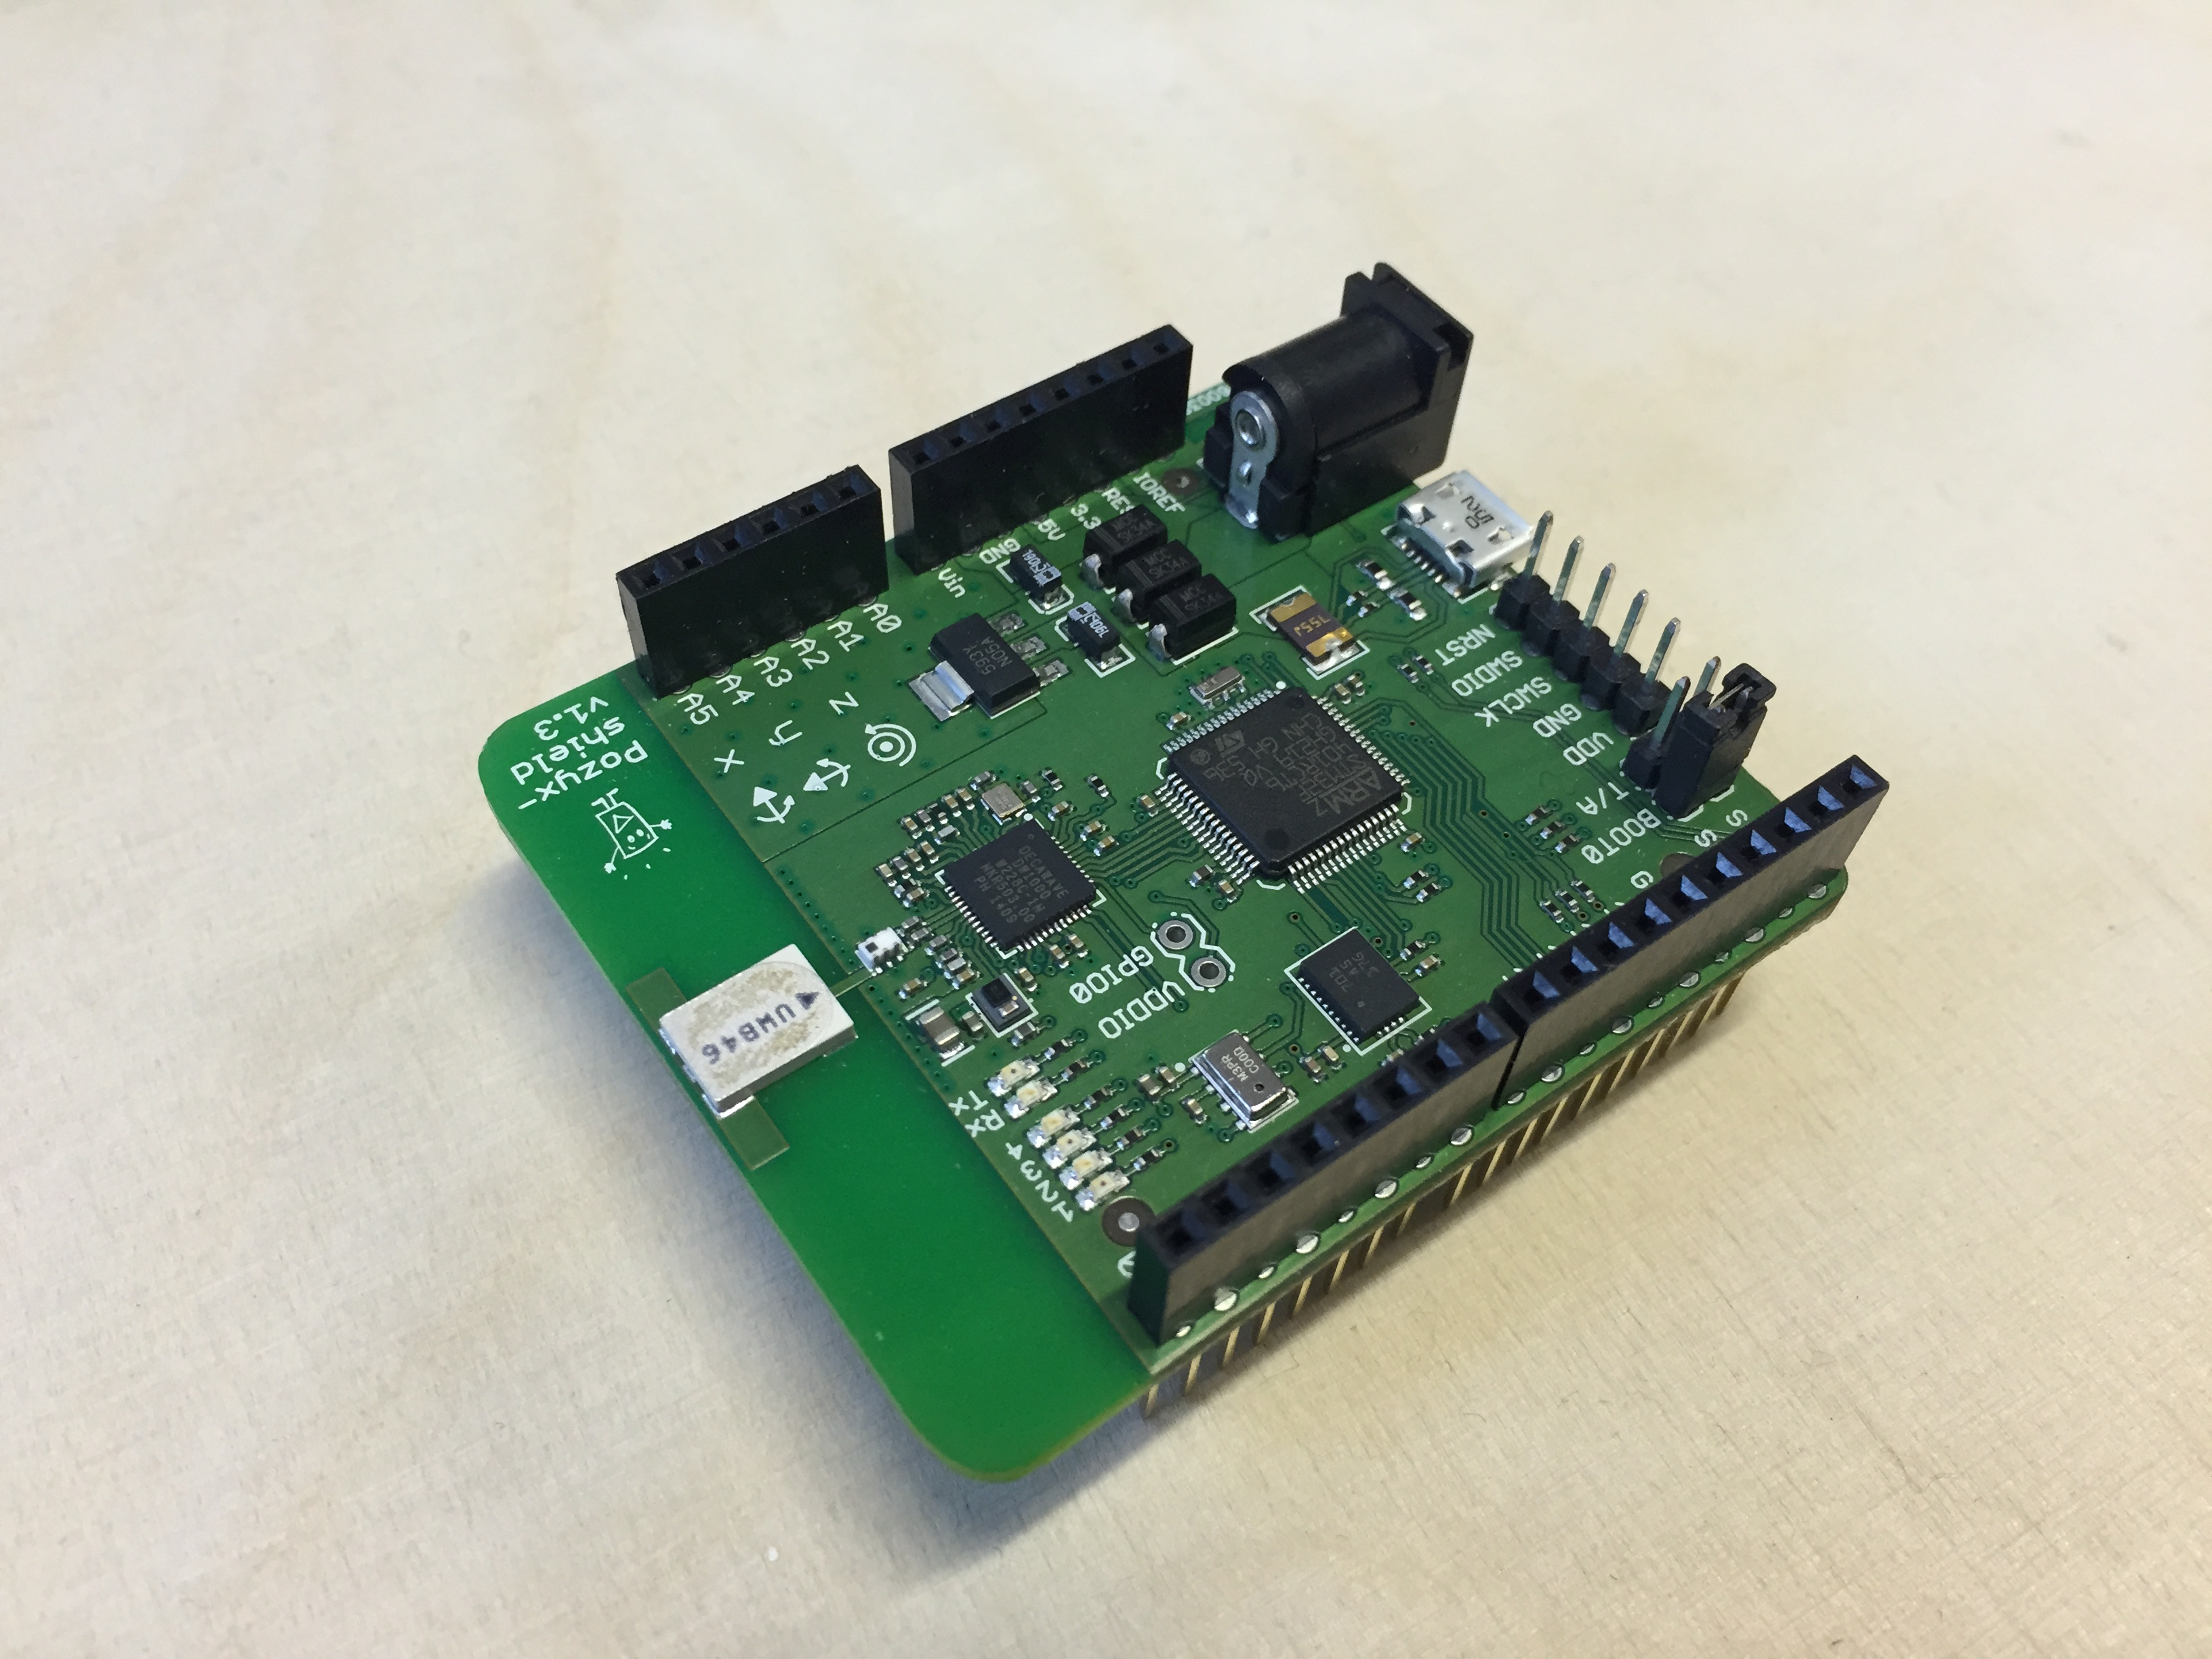
\includegraphics[width=0.5\linewidth]{../fig/pozyx_tag}
	\caption[Picture of Pozyx tag/anchor]{Picture of Pozyx tag/anchor (Photo: \url{http://pozyx.io})}
	\label{fig:pozyx_tag}
\end{figure}


\subsection{Arduino}
At a very early stage it was discussed as to whether it would be possible to create our own tracking devices using Arduino boards and soldering and connecting Bluetooth-antennas to them to create a Bluetooth-transmitter.
We soon discovered that this was a field neither of us had any experience with, and it would probably have taken far too much time to develop this solution.
The probability of us creating a product, in such a short time, that would be comparable to the available off-the-shelf products is also low.

\subsection{Estimote}
Another popular beacon manufacturer is Estimote who produces a variety of BLE beacons \citep{EstimoteInc.2018}.
Together with their beacons Estimote also supplies a Software Development Kit (SDK) which theoretically should make it easy to interact with the beacons, however, there are warnings against using these Beacons and SDK because of the many bugs and instabilities in the SDK, and they even dropped support for their old version of it to create a new one from scratch \citep{Saetre2017}.


\section{Summary}
This chapter has presented technologies used in this research and the reason they were chosen.

\onlyinsubfile{\bibliographystyle{chicago}}
\onlyinsubfile{\bibliography{../library}}
\end{document}
